\subsection{UC8 - Annullamento operazione}
\begin{figure}[H]
    \centering
    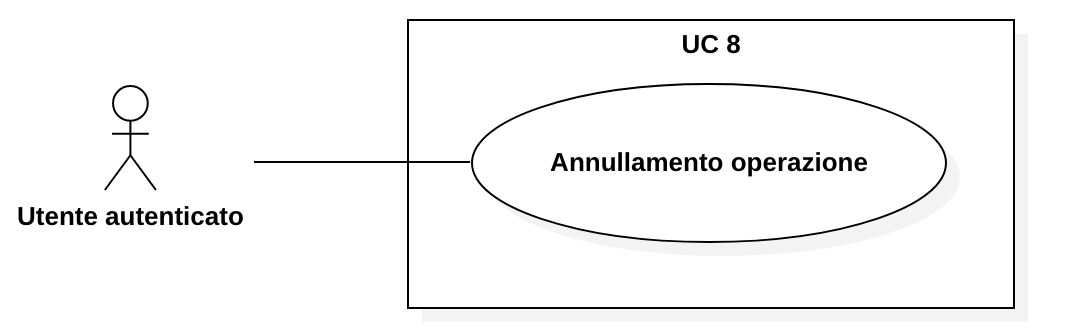
\includegraphics[scale = 0.7]{components/img/UC8.png}
    \caption{UC8 - Annullamento operazione}
\end{figure}
\begin{itemize}
\item \textbf{Attore Primario:} Utente autenticato;
\item \textbf{Precondizione:} L'utente ha a disposizione la possibilità di effettuare una selezione;
\item \textbf{Postcondizione:} Tutte le selezioni effettuate fino a quel momento vengono cancellate;
\item \textbf{Scenario principale:}
    \begin{enumerate}
    \item L'utente cambia idea sulle selezioni effettuate;
    \item Il sistema permette di cancellare ogni selezione fatta fino a quel momento cliccando sull'apposito pulsante.
    \end{enumerate}
\end{itemize}